\documentclass[]{article}
\usepackage{lmodern}
\usepackage{amssymb,amsmath}
\usepackage{ifxetex,ifluatex}
\usepackage{fixltx2e} % provides \textsubscript
\ifnum 0\ifxetex 1\fi\ifluatex 1\fi=0 % if pdftex
  \usepackage[T1]{fontenc}
  \usepackage[utf8]{inputenc}
\else % if luatex or xelatex
  \ifxetex
    \usepackage{mathspec}
  \else
    \usepackage{fontspec}
  \fi
  \defaultfontfeatures{Ligatures=TeX,Scale=MatchLowercase}
\fi
% use upquote if available, for straight quotes in verbatim environments
\IfFileExists{upquote.sty}{\usepackage{upquote}}{}
% use microtype if available
\IfFileExists{microtype.sty}{%
\usepackage{microtype}
\UseMicrotypeSet[protrusion]{basicmath} % disable protrusion for tt fonts
}{}
\usepackage[margin=1in]{geometry}
\usepackage{hyperref}
\hypersetup{unicode=true,
            pdftitle={DATA MINING IN R},
            pdfauthor={Carlvin Jerry},
            pdfborder={0 0 0},
            breaklinks=true}
\urlstyle{same}  % don't use monospace font for urls
\usepackage{graphicx,grffile}
\makeatletter
\def\maxwidth{\ifdim\Gin@nat@width>\linewidth\linewidth\else\Gin@nat@width\fi}
\def\maxheight{\ifdim\Gin@nat@height>\textheight\textheight\else\Gin@nat@height\fi}
\makeatother
% Scale images if necessary, so that they will not overflow the page
% margins by default, and it is still possible to overwrite the defaults
% using explicit options in \includegraphics[width, height, ...]{}
\setkeys{Gin}{width=\maxwidth,height=\maxheight,keepaspectratio}
\IfFileExists{parskip.sty}{%
\usepackage{parskip}
}{% else
\setlength{\parindent}{0pt}
\setlength{\parskip}{6pt plus 2pt minus 1pt}
}
\setlength{\emergencystretch}{3em}  % prevent overfull lines
\providecommand{\tightlist}{%
  \setlength{\itemsep}{0pt}\setlength{\parskip}{0pt}}
\setcounter{secnumdepth}{0}
% Redefines (sub)paragraphs to behave more like sections
\ifx\paragraph\undefined\else
\let\oldparagraph\paragraph
\renewcommand{\paragraph}[1]{\oldparagraph{#1}\mbox{}}
\fi
\ifx\subparagraph\undefined\else
\let\oldsubparagraph\subparagraph
\renewcommand{\subparagraph}[1]{\oldsubparagraph{#1}\mbox{}}
\fi

%%% Use protect on footnotes to avoid problems with footnotes in titles
\let\rmarkdownfootnote\footnote%
\def\footnote{\protect\rmarkdownfootnote}

%%% Change title format to be more compact
\usepackage{titling}

% Create subtitle command for use in maketitle
\newcommand{\subtitle}[1]{
  \posttitle{
    \begin{center}\large#1\end{center}
    }
}

\setlength{\droptitle}{-2em}

  \title{DATA MINING IN R}
    \pretitle{\vspace{\droptitle}\centering\huge}
  \posttitle{\par}
    \author{Carlvin Jerry}
    \preauthor{\centering\large\emph}
  \postauthor{\par}
      \predate{\centering\large\emph}
  \postdate{\par}
    \date{2019-01-25}


\begin{document}
\maketitle

\subsection{Getting started with Text mining using Twitter and
R}\label{getting-started-with-text-mining-using-twitter-and-r}

Social media usage has grown rapidly over the past few decades, most
social networks we can think of now are so well established, making them
a platform where people can not only talk to one another but also be
able to come forward with different views and interests they would like
to express. With an almost constant rate of increasing users each day,
social networks such as Facebook and Twitter have become great sources
of data which can be used in the broad field of Data Science:Talk of
(those pretty annoying) targeted ads for example, we all have such
moments online\ldots{}

\begin{figure}
\centering
\includegraphics{https://media.giphy.com/media/aE3DxYIBoSgaA/giphy.gif}
\caption{They just keep coming!!}
\end{figure}

With the help of APIs, we are easily able to get data from such
platforms to be used for further analysis. In this article we will go
through the first step of text mining in R using data fetched from
Twitter. The main advantage of these APIs is that the data we will fetch
comes in a well-structured format which makes our work easier when
crunching. In this case we will use the readily available Twitter API
and create our own Twitter app that will then help in fetching the data.
The following steps will accomplish the task\ldots{}

\subsubsection{Creating a Twitter app}\label{creating-a-twitter-app}

To create a twitter app we can use for fetching metadata, we first need
to have a Twitter account. We then need to go to the \textbf{twitter dev
site} \url{https://developer.twitter.com/} and log in with our user
account.

\begin{figure}
\centering
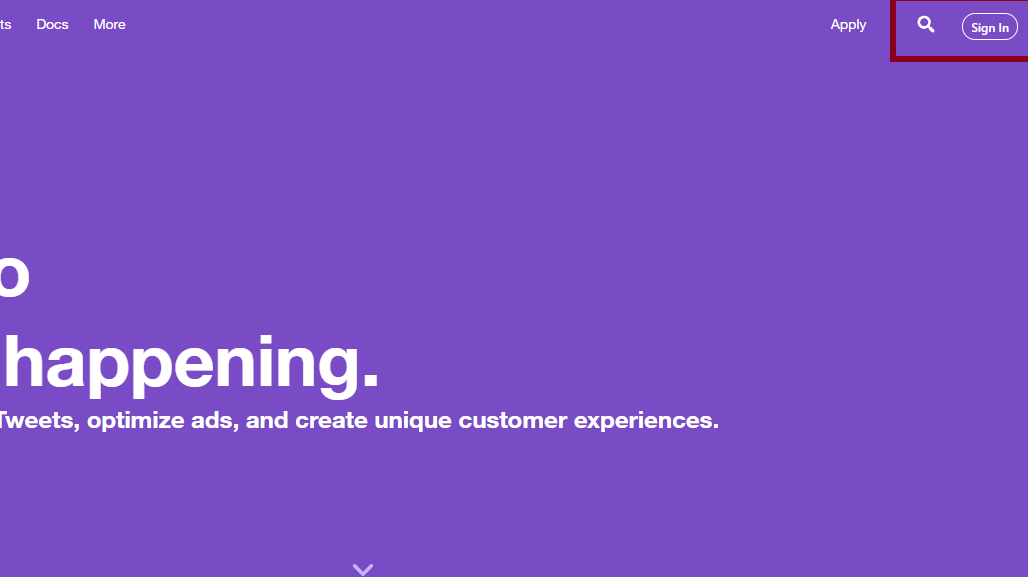
\includegraphics{/post/MyImages/login.png}
\caption{Login page}
\end{figure}

Next, on the top right corner should be a drop down menu next to your
username, go to APPS. At this point if you are doing this for the first
time your Apps section should be blank. Click on ``Create an app''
to\ldots{} create an app. 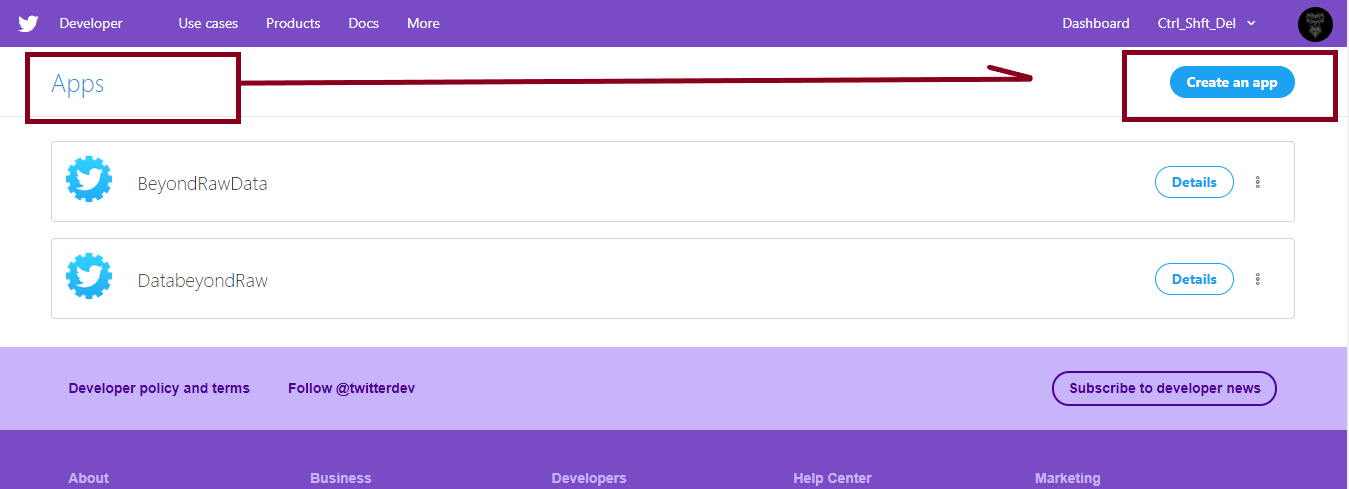
\includegraphics{/post/MyImages/apps.png}

We then then have to fill in the form bellow appropriately. Here is a
breakdown of what's required:

\begin{itemize}
\tightlist
\item
  \textbf{Name:} Give your app a unique name of your choice, e.g
  \textbf{UniqueName}
\item
  \textbf{Description:} This can always be changed later, use this to
  provide a brief note on what your app is all about to be able to
  distinguish it from other apps you might create in future.
\item
  \textbf{Website:} This should be your application's home page web
  site. It is however not applicable for most personal apps. Anything
  goes here e.g \url{https://carlvinjerry.github.io}
\item
  \textbf{Callback URL:} I would ignore the Callback URL field. If you
  are allowing users to log into your app to authenticate themselves,
  you'd enter the URL where they would be returned after they've given
  permission to Twitter to use your app.
  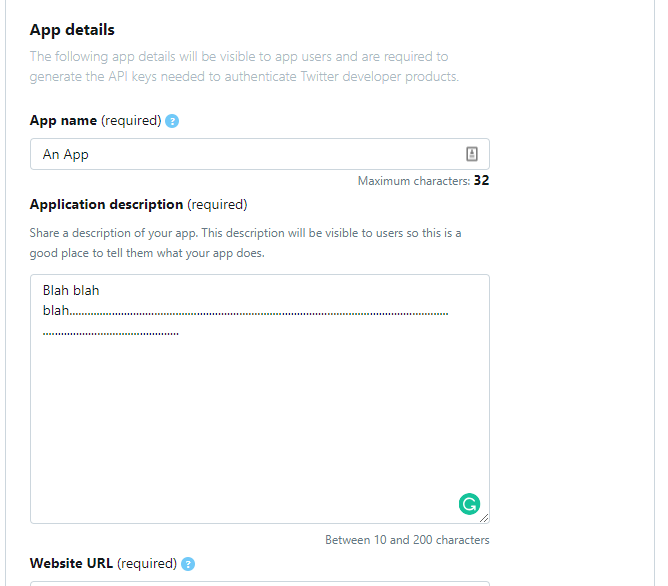
\includegraphics{/post/MyImages/apps2.png}
\end{itemize}

The remaining fields should be quite straight forward but must be
filled. Click ``Create'' once done and there you have your first twitter
app. On your app is a menu with \textbf{Keys and tokens}. These are the
most important components since we will need them to access data from
the APIs.Generate both consumer and access token if not preceent and
take note of them. \textbf{NB:} \textbf{These keys are meant for your
eyes only!}

\begin{figure}
\centering
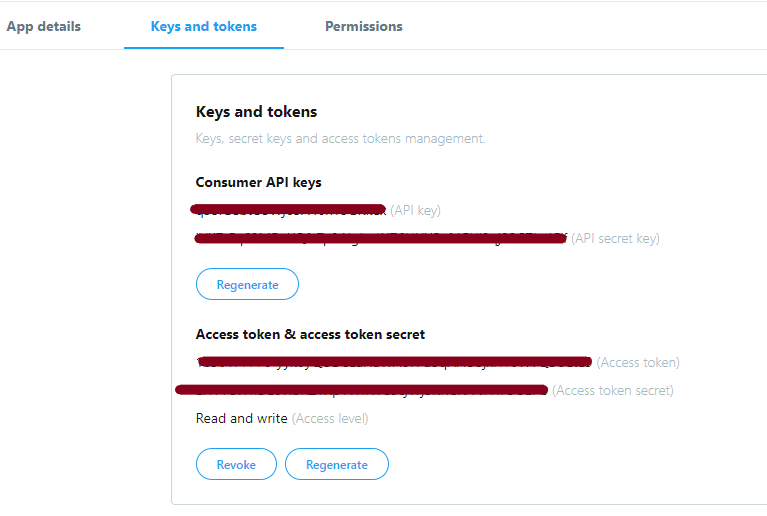
\includegraphics{/post/MyImages/keys.png}
\caption{API Keys}
\end{figure}

The final bit of setting up our twitter app is granting access
permissions. We will mostly do fine with the \textbf{read-only} if all
we need is to fetch data but it can always be changed later.

\begin{figure}
\centering
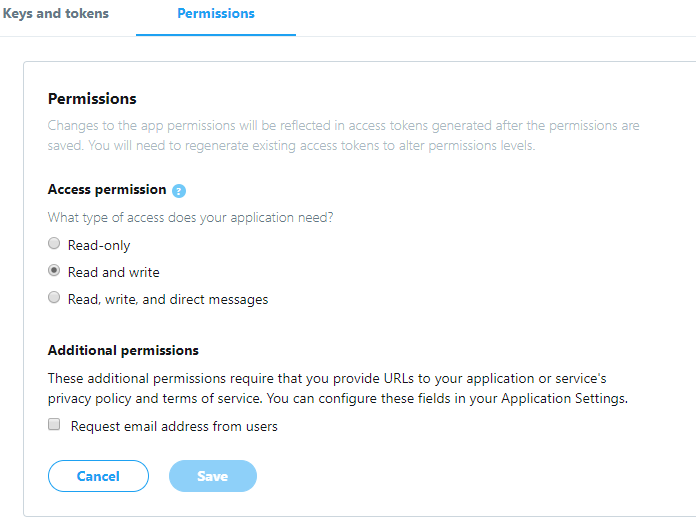
\includegraphics{/post/MyImages/permisions.png}
\caption{Permissions}
\end{figure}

Now we can move on to the next step where we set up \textbf{R} to query
data from Twitter.

\subsection{Setting up R to fetch twitter
data}\label{setting-up-r-to-fetch-twitter-data}


\end{document}
